
The concept of a stack has a long tradition, but stack machines no
longer form part of mainstream computers. Although stacks are no
longer used for expression evaluation, they are still used for the
context save on a function call. A niche language, Forth
\cite{Koopman89}, is stack-based and known as an efficient language
for controller applications. Some hardware implementations of the
Forth abstract machine do exist. These Forth processors are stack
machines.

The Java programming language defines not only the language but also
a binary representation of the program and an abstract machine, the
JVM, to execute this binary. The JVM is similar to the Forth
abstract machine in that it is also a stack machine. However, the
usage of the stack differs from Forth in such a way that a Forth
processor is not an ideal hardware platform to execute Java
programs.

In this section, the stack usage in the JVM is analyzed. We will see
that, besides the access to the top elements of the stack, an
additional access path to an arbitrary element of the stack is
necessary for an efficient implementation of the JVM. Two
architectures will be presented for this mixed access mode of the
stack. Both architectures are used in Java processors. However, we
will also show that the JVM does not need a full three-port access
to the stack as implemented in the two architectures. This allows
for a simple and more elegant design of the stack for a Java
processor. This proposed architecture will then be compared with the
other two at the end of this section.

\subsection{Java Computing Model}

The JVM is not a pure stack machine in the sense of, for instance,
the stack model in Forth. The JVM operates on a LIFO stack as its
\emph{operand stack}. The JVM supplies instructions to load values
on the operand stack, and other instructions take their operands
from the stack, operate on them and push the result back onto the
stack. For example, the \code{iadd} instruction pops two values from
the stack and pushes the result back onto the stack. These
instructions are the stack machine's typical zero-address
instructions. The maximum depth of this operand stack is known at
compile time. In typical Java programs, the maximum depth is very
small. To illustrate the operation notation of the JVM,
Table~\ref{tab_stack_not} shows the evaluation of an expression for
a stack machine notation and the JVM bytecodes. Instruction
\code{iload{\_}n} loads an integer value from a local variable at
position \emph{n} and pushes the value on TOS.

\begin{table}[htbp]
    \centering
    \begin{tabular}{ll}
        \toprule
        \multicolumn{2}{c}{\emph{A = B + C * D}}  \\
        \midrule
        Stack & JVM \\
        \midrule
        push B& iload{\_}1 \\
        push C& iload{\_}2 \\
        push D& iload{\_}3 \\
        {*}   & imul \\
        +     & iadd \\
        pop A & istore{\_}0 \\
        \bottomrule
    \end{tabular}
    \caption{Standard stack notation and the corresponding
    JVM instructions}
    \label{tab_stack_not}
\end{table}

The JVM contains another memory area for method local data. This
area is known as \emph{local variables}. Primitive type values, such
as integer and float, and references to objects are stored in these
local variables. Arrays and objects cannot be allocated in a local
variable, as in C/C++. They have to be placed on the heap. Different
instructions transfer data between the operand stack and the local
variables. Access to the first four elements is optimized with
dedicated single byte instructions, while up to 256 local variables
are accessed with a two-byte instruction and, with the \code{wide}
modifier, the area can contain up to 65536 values.

These local variables are very similar to registers and it appears
that some of these locals can be mapped to the registers of a
general purpose CPU or implemented as registers in a Java processor.
On method invocation, local variables could be saved in a frame on a
stack, different from the operand stack, together with the return
address, in much the same way as in C on a typical processor. This
would result in the following memory hierarchy:
%
\begin{itemize}
\item On-chip hardware stack for ALU operations
\item A small register file for frequently-accessed variables
\item A method stack in main memory containing the return address and additional
local variables
\end{itemize}
%
However, the semantics of method invocation suggest a different
model. The arguments of a method are pushed on the operand stack. In
the invoked method, these arguments are not on the operand stack but
are instead accessed as the first variables in the local variable
area. The \emph{real} method local variables are placed at higher
indices. Listing~\ref{lst:stack:param:pass} gives an example of the
argument passing mechanism in the JVM. These arguments could be
copied to the local variable area of the invoked method. To avoid
this memory transfer, the entire variable area (the arguments
\emph{and} the variables of the method) is allocated on the operand
stack. However, in the invoked method, the arguments are buried deep
in the stack.

\begin{lstlisting}[float,caption={Example of parameter passing and access},label={lst:stack:param:pass}]
The Java source:

    int val = foo(1, 2);
    ...
    public int foo(int a, int b) {
        int c = 1;
        return a+b+c;
    }

Compiled bytecode instructions for the JVM:

The invocation sequence:
    aload_0             // Push the object reference
    iconst_1            // and the parameter onto the
    iconst_2            // operand stack.
    invokevirtual   #2  // Invoke method foo:(II)I.
    istore_1            // Store the result in val.

public int foo(int,int):
    iconst_1            // The constant is stored in a method
    istore_3            // local variable (at position 3).
    iload_1             // Arguments are accessed as locals
    iload_2             // and pushed onto the operand stack.
    iadd                // Operation on the operand stack.
    iload_3             // Push c onto the operand stack.
    iadd
    ireturn             // Return value is on top of stack.
\end{lstlisting}

This asymmetry in the argument handling prohibits passing down
parameters through multiple levels of subroutine calls, as in Forth.
Therefore, an extra stack for return addresses is of no use for the
JVM. This single stack now contains the following items in a frame
per method:
%
\begin{itemize}
\item The local variable area
\item Saved context of the caller
\item The operand stack
\end{itemize}
%
A possible implementation of this layout is shown in
Figure~\ref{fig_stack_invoke}. A method with two arguments,
\code{arg{\_}1} and \code{arg{\_}2} (\code{arg{\_}0} is the
\emph{this} pointer), is invoked in this example. The invoked method
\emph{sees} the arguments as \code{var{\_}1} and \code{var{\_}2}.
\code{var{\_}3} is the only local variable of the method. SP is a
pointer to the top of the stack and VP points to the start of the
variable area.

\begin{figure}
    \centering
    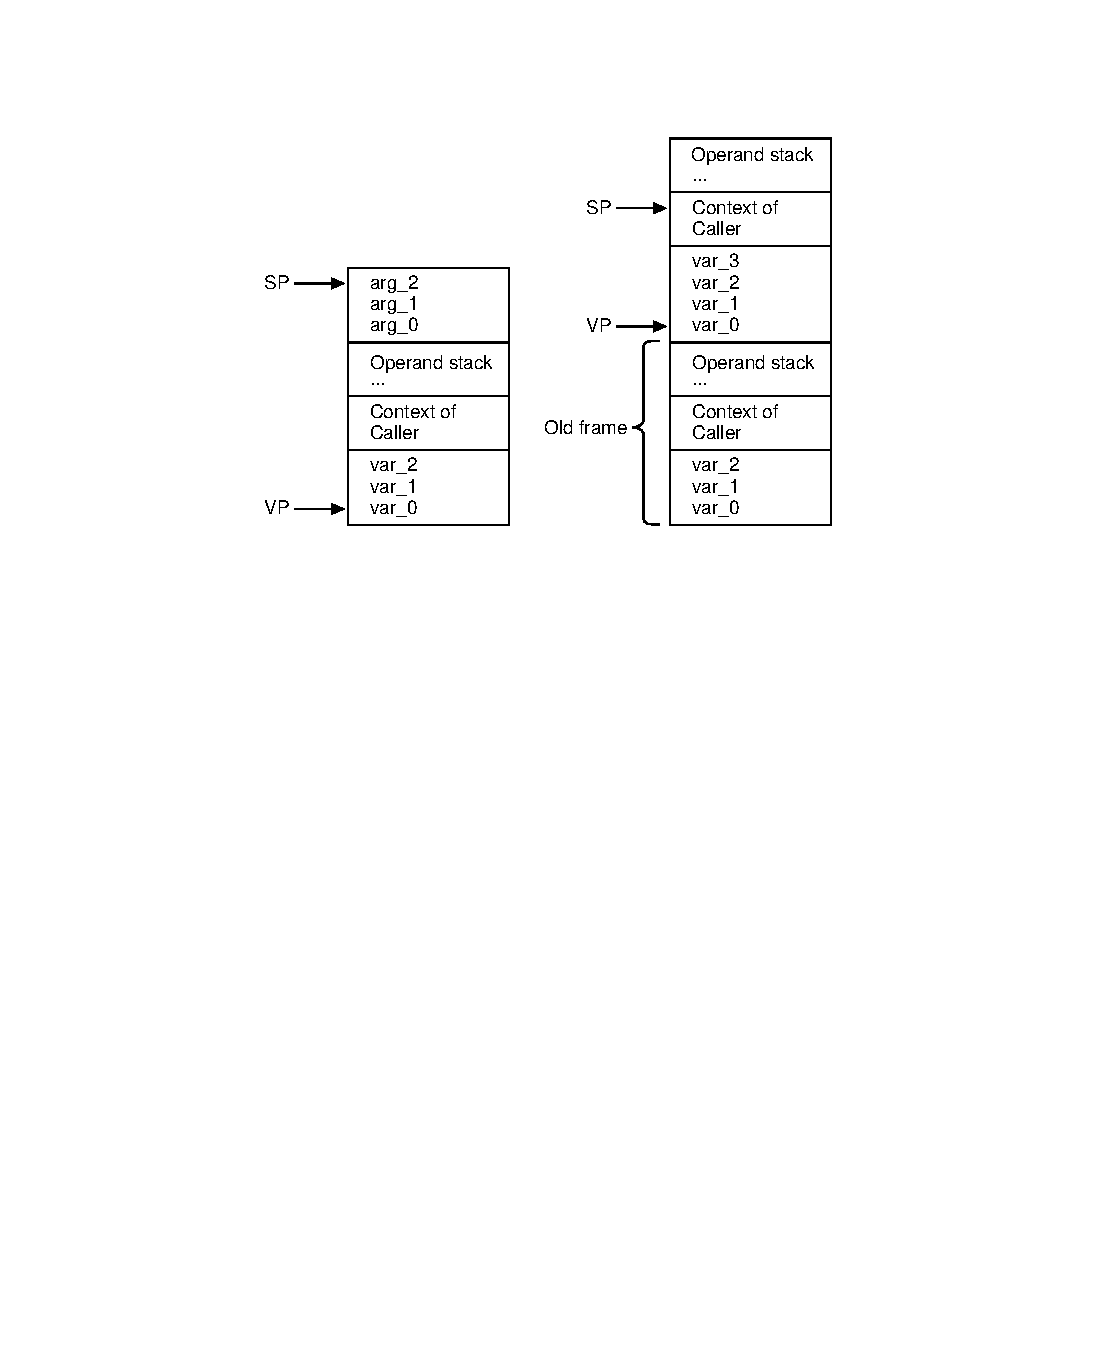
\includegraphics[scale=\picscale]{stack/stack_invocation}
    \caption{Stack change on method invocation}
    \label{fig_stack_invoke}
\end{figure}

\subsection{Access Patterns on the Java Stack}
\label{subsec:access}

The pipelined architecture of a Java processor executes basic
instructions in a single cycle. A stack that contains the operand
stack \emph{and} the local variables results in the following access
patterns:
%
\begin{description}
\item[Stack Operation:] Read of the two top elements, operate on them and
push back the result on the top of the stack. The pipeline stages
for this operation are:\newline
\texttt{
    value1 $\leftarrow $ stack[sp], value2 $\leftarrow $ stack[sp-1]\newline
    result $\leftarrow $ value1 op value2, sp $\leftarrow $ sp-1\newline
    stack[sp] $\leftarrow $ result
}

\item[Variable Load:] Read a data element deeper down in the
    stack, relative to a variable base address pointer (VP), and
    push this data on the top of the stack. This operation needs
    two pipeline stages:\newline \texttt{ value $\leftarrow $
    stack[vp+offset], sp $\leftarrow $ sp+1\newline stack[sp]
    $\leftarrow $ value
}

\item[Variable Store:] Pop the top element of the stack and write it in
the variable relative to the variable base address:\newline
\texttt{
    value $\leftarrow $ stack[sp]\newline
    stack[vp+offset] $\leftarrow $ value, sp $\leftarrow $ sp-1
}
\end{description}
%
For pipelined execution of these operations, a three-port memory or
register file (two read ports and one write port) is necessary.

\subsection{Common Realizations of a Stack Cache}

As the stack is a heavily accessed memory region, the stack -- or
part of it -- has to be placed in the upper level of the memory
hierarchy. This part of the stack is referred to as a \emph{stack
cache}. As described in \cite{Hennessy02}, a typical memory hierarchy
contains the following elements, with increasing access time and
size:
%
\begin{itemize}
\item CPU register
\item On-chip cache memory
\item Off-chip cache memory
\item Main memory
\item Magnetic disk for virtual memory
\end{itemize}
%
For a stack cache, a register file is the solution with the shortest access
time. However, in order to store more than a few elements in the cache, an
on-chip memory realization can provide a larger cache. Both variants have
been used and are described below.

\subsubsection{The Register File as a Stack Cache}

An example of a Java processor that uses a register file is Sun's
picoJava \cite{pjMicroArch}. It contains 64 registers, organized as a
circular buffer. To compensate for this \emph{small} stack cache, an
automatic spill and fill circuit needs another read/write port to the
register file. aJile's JEMCore \cite{880720} is a direct-execution
Java processor core that contains 24 registers. Only six of them are
used to cache the top elements of the stack. With this small register
count, local variables are not part of the cache. Ignite
\cite{IGNITE} (formerly known as PSC1000) is a stack processor,
originally designed as a Forth processor and now promoted as a Java
processor, and has an operand stack that contains 18 registers with
automatic spill and fill.

A basic pipeline for a stack processor with a register file contains the
following stages:
%
\begin{enumerate}
\item IF -- instruction fetch
\item ID -- instruction decode
\item EX -- read register file and execute
\item WB -- write result back to register file
\end{enumerate}
%
With this pipeline structure, a single data-forwarding path between
WB and EX is necessary. The ALU with the register file (with a size
of 16, a common size for RISC processors) and the bypass unit are
shown in Figure~\ref{fig_stack_cache_reg}. In
Table~\ref{tab_resource_reg_cache} the hardware resources of this
type of stack cache are approximated, using the values given in
Table~\ref{tab_simp_gate_count} (a MUX not found in this table is
assumed to use combinations of the basic types; e.g.\ two 8:1 and
one 2:1 for a 16:1). An experimental evaluation of this architecture
in an FPGA is described in Section~\ref{subsec:resource}.

\begin{table}[hbtp]
    \centering
    \begin{tabular}{lc}
        \toprule
        Basic function & Gate count \\
        \midrule
        D-Flip-Flop&5 \\
        2:1 MUX&3 \\
        4:1 MUX&5 \\
        8:1 MUX&9 \\
        SRAM Bit&1.5 \\
        \bottomrule
    \end{tabular}
    \caption{Simplified gate count for basic functions}
    \label{tab_simp_gate_count}
\end{table}

\begin{figure*}
    \centering
    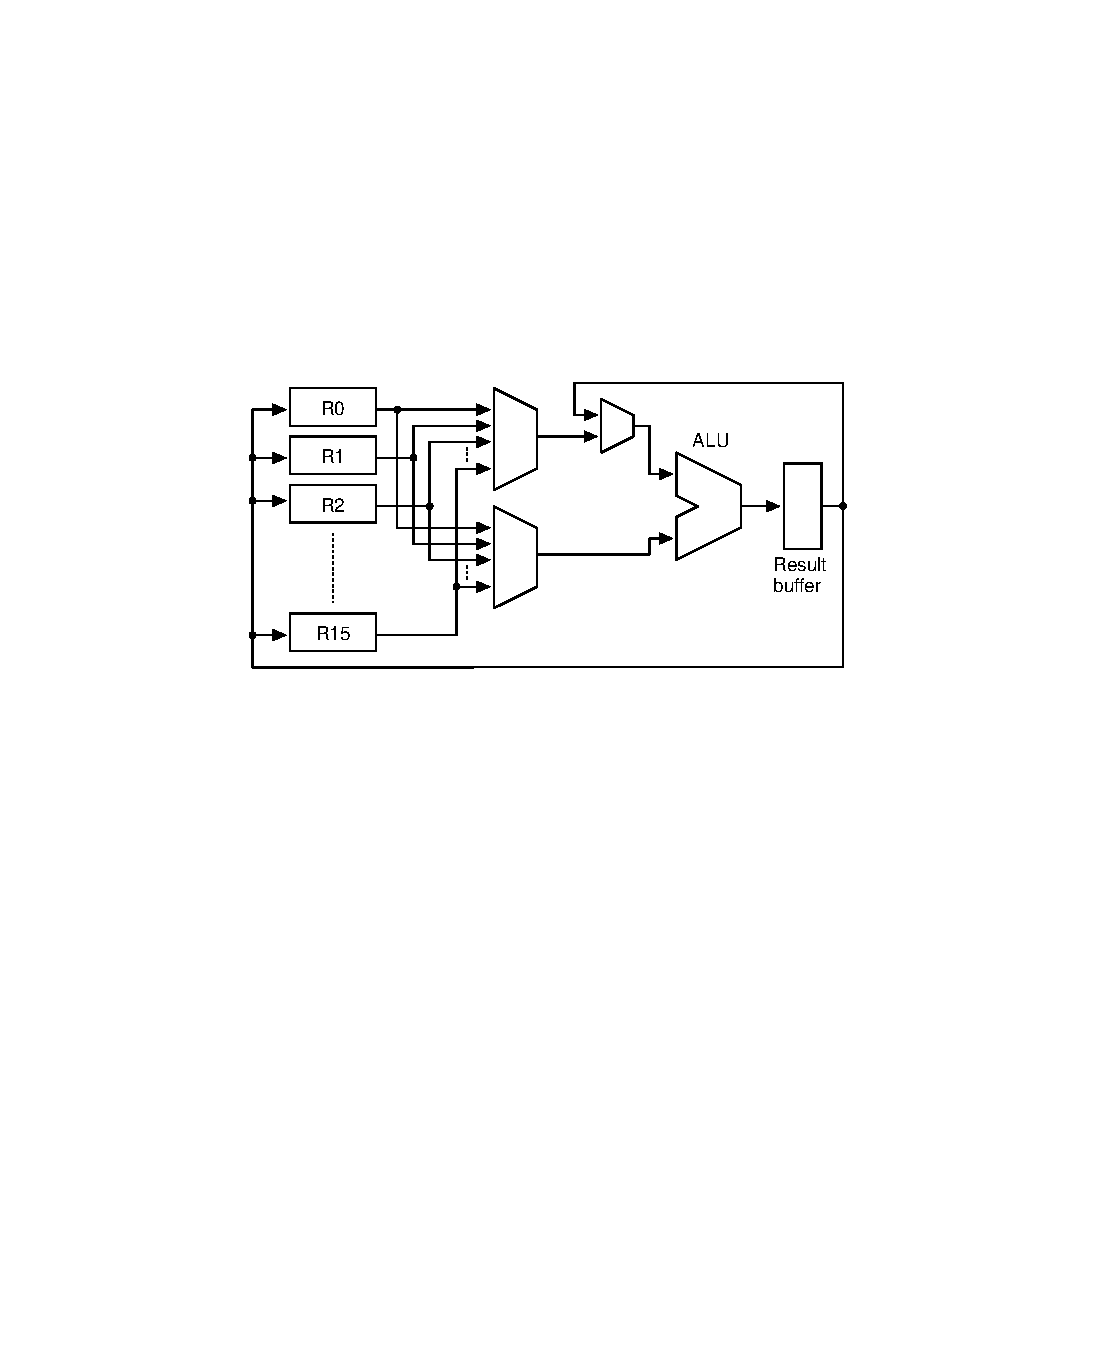
\includegraphics[scale=\picscale]{stack/stack_cache_reg}
    \caption{A stack cache with registers}
    \label{fig_stack_cache_reg}

    \vspace{\floatsep}    % zusaetzlicher Abstand zwischen zwei `floats'

    \begin{tabular}{lld{1}}
        \toprule
        Function block& Basic function& \cc{Gate count} \\
        \midrule
        Register File& 512 D-Flip-Flops& 2,560 \\
        Read MUX& 2x32 16:1 MUX&1,344 \\
        Forward MUX& 32 2:1 MUX&96 \\
        ALU buffer& 32 D-Flip-Flops&160 \\
        \midrule
        \textbf{Total}& &4,160 \\
        \bottomrule
    \end{tabular}
    \captionof{table}{Estimated gate count for a register stack cache}
    \label{tab_resource_reg_cache}
\end{figure*}

\subsubsection{On-chip Memory as a Stack Cache}

Using SRAM on the chip provides a \emph{large} stack cache (e.g.\
128 entries). However, as we have seen in
Section~\ref{subsec:access}, a three-port memory is necessary. An
additional pipeline stage performs the cache memory read:
%
\begin{enumerate}
\item IF -- instruction fetch
\item ID -- instruction decode
\item RD -- memory read
\item EX -- execute
\item WB -- write result back to memory
\end{enumerate}
%
With this pipeline structure, two data forwarding paths are
necessary. The resulting architecture is shown in
Figure~\ref{fig_stack_cache_ram} and a gate count estimate is
provided in Table~\ref{tab_resource_sram_cache}. This version needs
70{\%} more resources than the first one, but provides an eight
times larger stack cache.

Example designs that use this kind of stack cache are (i) Komodo
\cite{Zulauf00}, a Java processor intended as a basis for research
on multithreaded real-time scheduling, and (ii) FemtoJava
\cite{Femto01}, a research project to build an application specific
Java processor.

A three-port memory is an expensive option for an ASIC and unusual
in an FPGA. It can be emulated in an FPGA by two memories with a
single read and write port. The write data is written in both memory
blocks and each memory block provides a different read port.
However, this solution also doubles the amount of memory.

Both designs (Komodo and FemtoJava) avoid the memory doubling by
serializing the two reads. This serialization results in a minimum of
two clock cycles execution time for basic instructions or halves the
clock frequency of the whole pipeline.

\begin{figure*}
    \centering
    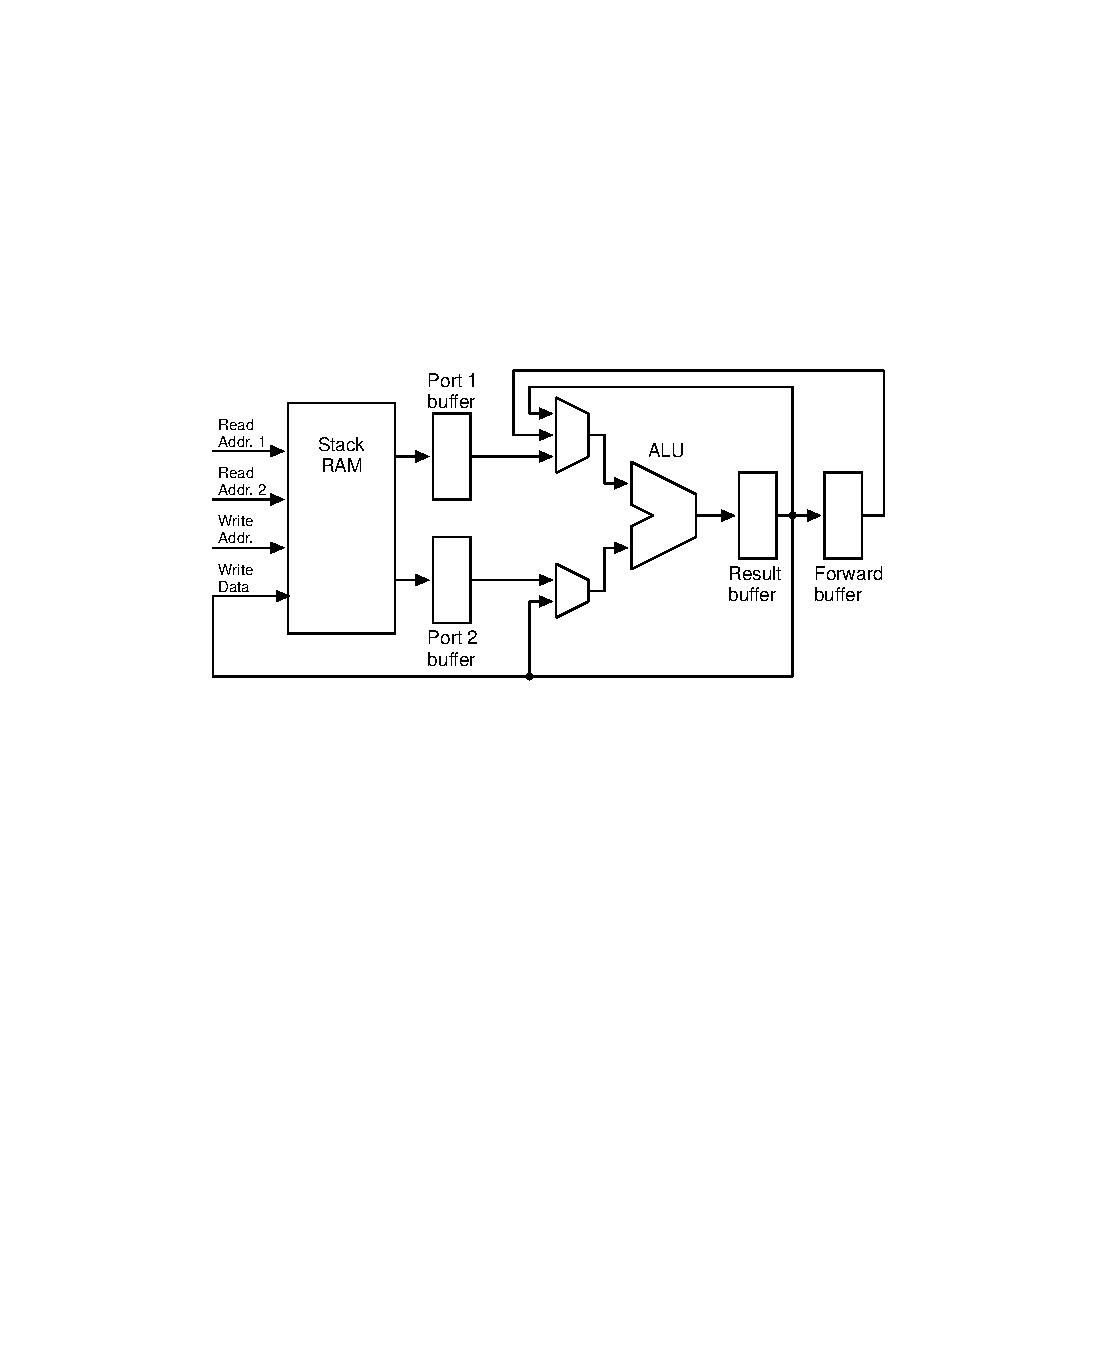
\includegraphics[scale=\picscale]{stack/stack_cache_ram}
    \caption{A stack cache with on-chip RAM}
    \label{fig_stack_cache_ram}

    \vspace{\floatsep}    % zusaetzlicher Abstand zwischen zwei `floats'

    \begin{tabular}{lld{1}}
        \toprule
        Function block& Basic function& \cc{Gate count} \\
        \midrule
        Stack RAM& e.g.\ 128x32 Bits& 6,144 \\
        Port buffer& 2x32 D-Flip-Flops& 320 \\
        Forward MUX& 32x 2:1 MUX, 3:1 MUX& 288 \\
        ALU buffer& 2x32 D-Flip-Flops& 320 \\
        \midrule
        \textbf{Total}& & 7,072 \\
        \bottomrule
    \end{tabular}
    \captionof{table}{Estimated gate count for a stack cache with RAM}
    \label{tab_resource_sram_cache}
\end{figure*}

\subsection{A Two-Level Stack Cache}

In this section, we will discuss access patterns of the JVM and
their implication on the functional units of the pipeline. A faster
and smaller architecture is proposed for the stack cache of a Java
processor.

\subsubsection{JVM Stack Access Revised}

If we analyze the JVM's access patterns to the stack in more detail,
we can see that a two-port read is only performed with the two top
elements of the stack. All other operations with elements deeper in
the stack, local variables load and store, only need one read port.
If we only implement the two top elements of the stack in registers,
we can use a standard on-chip RAM with one read and one write port.

We will show that all operations can be performed with this
configuration. Let $A$ be the top-of-stack, $B$ the element below
top-of-stack. The memory that serves as the second level cache is
represented by the array $sm$. Two indices in this array are used:
$p$ points to the logical third element of the stack and changes as
the stack grows or shrinks, $v$ points to the base of the local
variables area in the stack and $n$ is the address offset of a
variable. $op$ is a two operand stack operation with a single result
(i.e.\ a typical ALU operation).


\begin{description}
\begin{samepage}
\item[Case 1:]
ALU operation \newline \textit{A $\leftarrow $ A op B
\newline B $\leftarrow $ sm[p] \newline p $\leftarrow $ p -- 1
\newline }The two operands are provided by the two top level
registers. A single read access from $sm$ is necessary to fill $B$
with a new value.
\end{samepage}
%
\begin{samepage}
\item[Case 2:]
    Variable load (\textit{Push}) \newline
    \textit{
    sm[p+1]$\leftarrow $ B \newline
    B $\leftarrow $ A \newline
    A$\leftarrow $ sm[v+n] \newline
    p $\leftarrow $ p + 1 \newline
    }
    One read access from \textit{sm} is necessary for the variable read. The
former TOS value moves down to $B$ and the data previously in $B$ is
written to \textit{sm}.
\end{samepage}
%
\begin{samepage}
\item[Case 3:]
    Variable store (\textit{Pop}) \newline
    \textit{sm[v+n] $\leftarrow $ A \newline
    A $\leftarrow $ B \newline
    B $\leftarrow $ sm[p] \newline
    p $\leftarrow $ p - 1 \newline }
    The TOS value is written to \textit{sm}. $A$ is filled with $B$ and $B$ is filled in an
identical manner to Case 1, needing a single read access from
\textit{sm}.
\end{samepage}
\end{description}
%
We can see that all three basic operations can be performed with a
stack memory with one read and one write port. Assuming a memory is
used that can handle concurrent read and write access, there is no
structural access conflict between $A$, $B$ and \textit{sm}. That
means that all operations can be performed concurrently in a single
cycle.

As we can see in Figure~\ref{fig_stack_invoke} the operand stack and
the local variables area are distinct regions of the stack. A
concurrent read from and write to the stack is only performed on a
variable load or store. When the read is from the local variables
area the write goes to the operand area; a read from the operand
area is concurrent with a write to the local variables area.
Therefore there is no concurrent read and write to the same location
in \textit{sm}. There is no constraint on the read-during-write
behavior of the memory (old data, undefined or new data), which
simplifies the memory design. In a design where read and write-back
are located in different pipeline stages, as in the architectures
described above, either the memory must provide the new data on a
read-during-write, or external forward logic is necessary.

From the three cases described, we can derive the memory addresses
for the read and write port of the memory, as shown in
Table~\ref{tab_stack_address}.

\begin{table}[htbp]
    \centering
    \begin{tabular}{cc}
        \toprule
        Read address&Write address \\
        \midrule p&p+1 \\
        v+n&v+n \\
        \bottomrule
    \end{tabular}
    \caption{Stack memory addresses}
    \label{tab_stack_address}
\end{table}

\subsubsection{The Datapath}

The architecture of the two-level stack cache can be seen in
Figure~\ref{fig_stack_cache_jop}. Register $A$ represents the
top-of-stack and register $B$ the data below the top-of-stack. ALU
operations are performed with these two registers and the result is
placed in $A$. During such an ALU operation, $B$ is filled with new
data from the stack RAM. A new value from the local variable area is
loaded directly from the stack RAM into $A$. The data previously in
$A$ is moved to $B$ and the data from $B$ is spilled to the stack
RAM. $A$ is stored in the stack RAM on a store instruction to the
local variable. The data from $B$ is moved to $A$ and $B$ is filled
with a new value from the stack RAM.
%All these operations are performed concurrently in one cycle.

With this architecture, the pipeline can be reduced to three stages:
%
\begin{enumerate}
\item IF -- instruction fetch
\item ID -- instruction decode
\item EX -- execute, load or store
\end{enumerate}
%
The estimated resource usage of this two-level stack cache
architecture is given in Table~\ref{tab_resource_jop_cache}. It can
be seen that this architecture is roughly as complex as the solution
given above (about 5{\%} less gates). However, the reduced
complexity with the two-port RAM instead of a three-port RAM is not
included in the table. The critical path through the ALU contains
only one 2:1 MUX to register $A$ in this solution, rather than one
3:1 MUX in one ALU path and one 2:1 MUX in the other ALU path. As no
data forwarding logic is necessary, the decoding logic is also
simpler.

\begin{figure*}
    \centering
    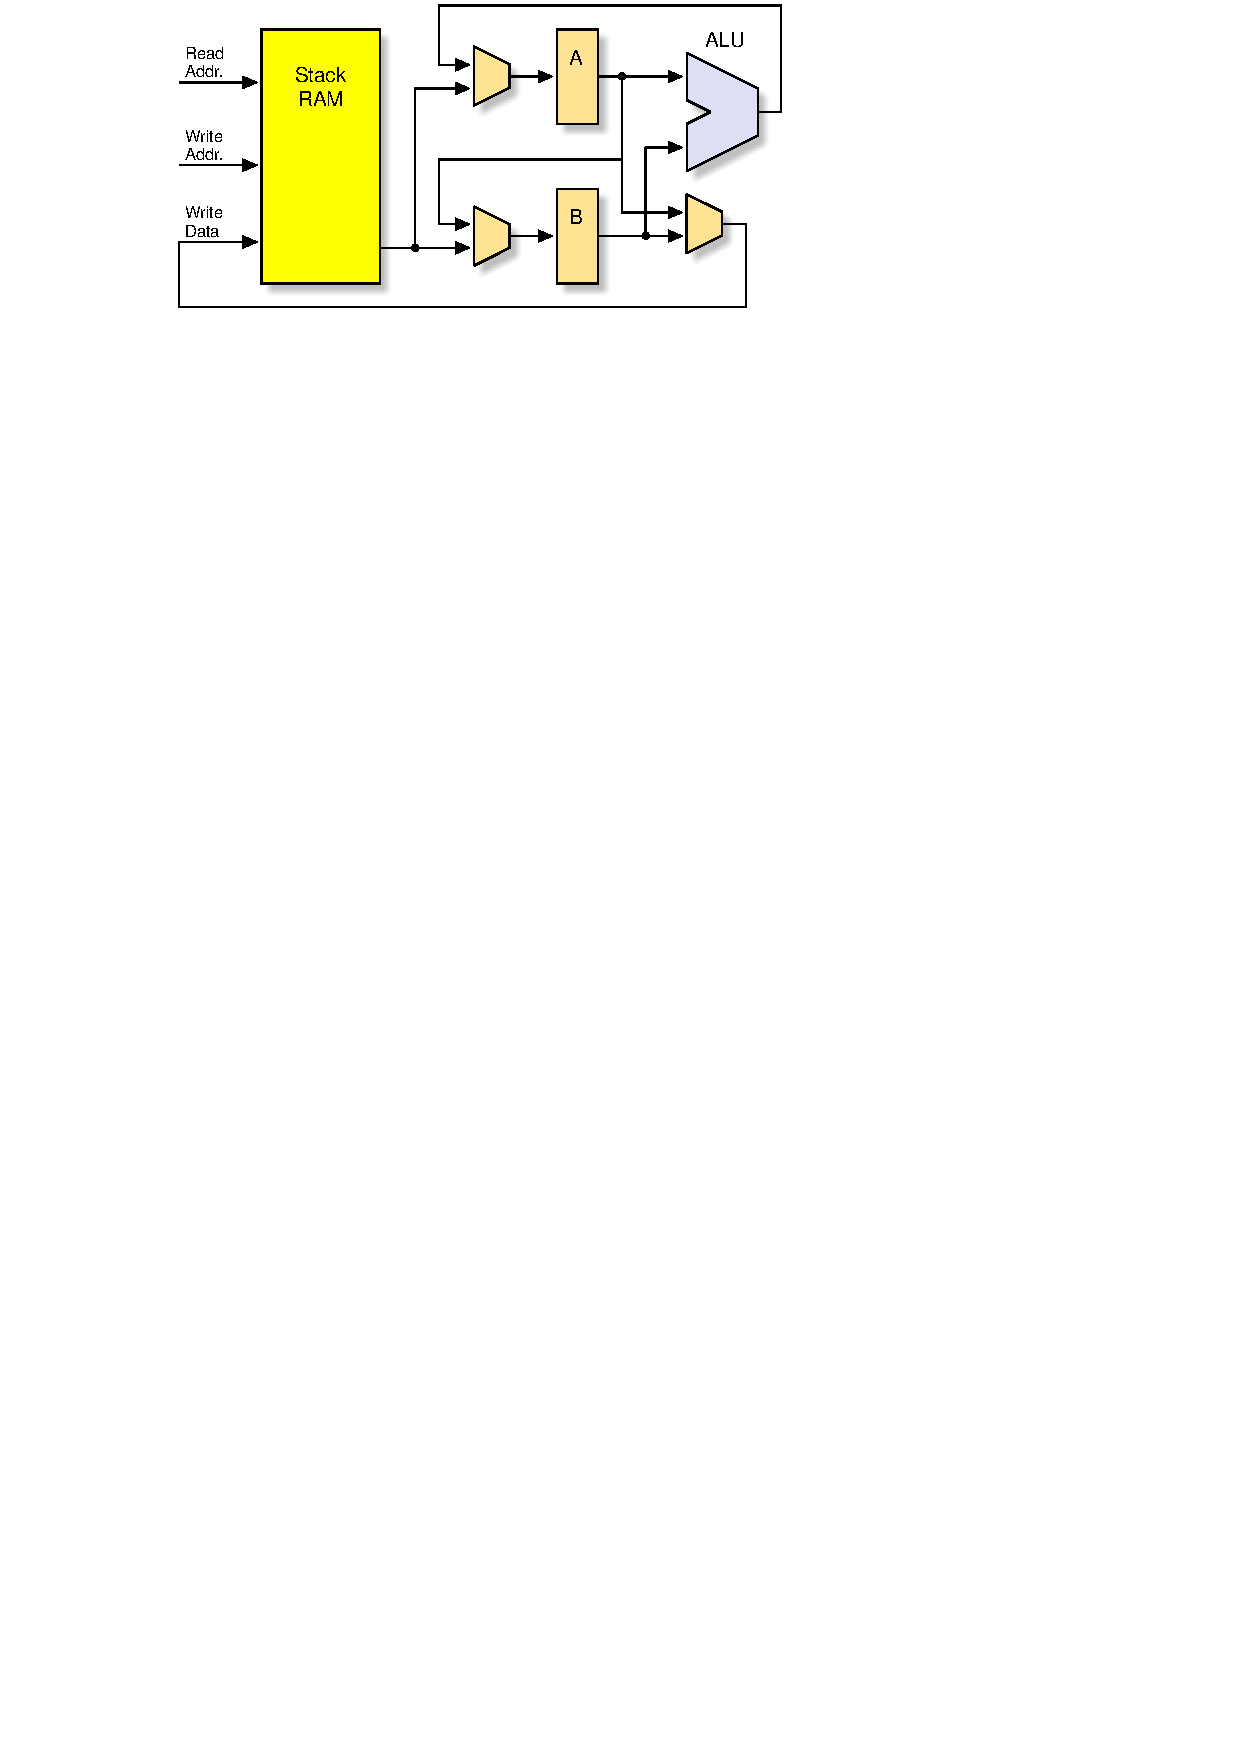
\includegraphics[scale=\picscale]{stack/stack_cache_jop}
    \caption{Two-level stack cache}
    \label{fig_stack_cache_jop}

    \vspace{\floatsep}    % zusaetzlicher Abstand zwischen zwei `floats'

    \begin{tabular}{lld{1}}
        \toprule
        Function block& Basic function& \cc{Gate count} \\
        \midrule
        Stack RAM& e.\ g.\ 128x32 Bits&6,144 \\
        TOS, TOS-1 buffer& 2x32 D-Flip-Flops&320 \\
        Three MUX& 3x32 2:1 MUX&288 \\
        \midrule
        \textbf{Total}& &6,752 \\
        \bottomrule
    \end{tabular}
    \captionof{table}{Estimated gate count for a two-level stack cache}
    \label{tab_resource_jop_cache}
\end{figure*}

\subsubsection{Data Forwarding -- A Non-Issue}

Data dependencies in the instruction stream result in the so-called
\emph{data hazards} \cite{Hennessy02} in the pipeline. Data
forwarding is a technique that moves data from a later pipeline
stage back to an earlier one to solve this problem. The term
\emph{forward} is correct in the temporal domain as data is
transferred to an instruction in the future. However, it is
misleading in the structural domain as the forward direction is
towards the \emph{last} pipeline stage for an instruction.

As the probability of data dependency is very high in a stack-based
architecture, one would expect several data forwarding paths to be
necessary. However, in the two-level architecture proposed, with its
resulting three-stage pipeline, no data hazards will occur and no
data forwarding is therefore necessary. This simplifies the decoding
stage and reduces the number of multiplexers in the execution path.
We will show that none of the three data hazard types
\cite{Hennessy02} is an issue in this architecture. With instructions
$i$ and $j$, where $i$ is issued before $j$, the data hazard types
are:

\paragraph{Read after write:} $j$ reads a source before $i$ writes it. This
is the most common type of hazard and, in the architectures
described above, is solved by using the ALU buffers and the
forwarding multiplexer in the ALU datapath. On a stack architecture,
write takes three forms:
%
\begin{itemize}
    \item Implicit write of TOS during an ALU operation
    \item Write to the TOS during a load instruction
    \item Write to an arbitrary entry of the stack with a store instruction
\end{itemize}
%
A read also occurs in three different forms:
\begin{itemize}
    \item Read two top values from the stack for an ALU operation
    \item Read TOS for a store instruction
    \item Read an arbitrary entry of the stack with the load instruction
\end{itemize}
%
With the two top elements of the stack as discrete registers, these
values are read, operated on and written back in the same cycle. No
read that depends on TOS or TOS-1 suffers from a data hazard. Read
and write access to a local variable is also performed in the same
pipeline stage. Thus, the read after write order is not affected.
However, there is also an additional hidden read and write: the fill
and spill of register B:



%
\begin{itemize}
\item \textit{B fill:}
$B$ is written during an ALU operation and on a variable store.
During an ALU operation, the operands are the values from $A$ and
the old value from $B$. The new value for $B$ is read from the stack
memory and does not depend on the new value of $A$. During a
variable store operation, $A$ is written to the stack memory and
does not depend on $B$. The new value for $B$ is also read from the
stack memory and it is not obvious that this value does not depend
on the written value. However, the variable area and the operand
stack are distinct areas in the stack (this changes only on method
invocation and return), guaranteeing that concurrent read/write
access does not produce a data hazard.

\item \textit{B spill:}
$B$ is read on a load operation. The new value of $B$ is the old
value of $A$ and does not therefore depend on the stack memory read.
$B$ is written to the stack. For the read value from the stack
memory that goes to $A$, the argument concerning the distinct stack
areas in the case of \textit{B fill} described above still applies.
\end{itemize}
%
\paragraph{Write after read:} $j$ writes a destination before it is read by
$i$. This cannot take place as all reads and writes are performed in
the same pipeline stage keeping the instruction order.

\paragraph{Write after write:} $j$ writes an operand before it is written by
$i$. This hazard is not present in this architecture as all writes
are performed in the same pipeline stage.



\subsection{Resource Usage Compared}
\label{subsec:resource}

The three architectures described above are implemented in Altera's
EP1C6Q240C6 \cite{AltCyc} FPGA. The three-port memory for the second
solution is emulated with two embedded memory blocks. The ALU for
this comparison is kept simple with the following functions: NOP,
ADD, SUB, POP, AND, OR, XOR and load external data. The load of
external data is necessary in order to prevent the synthesizer from
optimizing away the whole design. A real implementation of an ALU
for a Java processor, as described in Section~\ref{sec:pipeline}, is
a little bit more complex with a barrel shifter and additional load
paths. In order to gain the maximum operating frequency for the
design, the testbed for this architecture contains registers for the
external data, the RAM address buses, and the control and select
signals. Table~\ref{tab_stack_resources} shows the resource usage
and maximum operation frequency of the three different
architectures.

\begin{table*}
    \centering
    \begin{tabular}{lccccccc}
        \toprule
        Design& \multicolumn{2}{c}{Total}&
        \multicolumn{2}{c}{Cache}&
        Memory& fmax & Size\\
         & LCs& Reg.& LCs&
        Reg.& (bit)& (MHz) & (word)\\
        \midrule
%        ALU only& 194& 0& -& -& -&- &-\\
        Testbed w.\ ALU& 261& 166& -& -& -&237 & - \\
        16 register cache& 968& 657& 707& 491& 0&110 & 16 \\
%        16 Register cache& 297& 140& 36& -26& 1024&113 & 16 \\
        SRAM cache& 372& 185& 111& 19& 8,192&153 & 128\\
        Two-level cache& 373& 184& 112& 18& 4,096& 213 & 130\\
        \bottomrule
    \end{tabular}
    \caption{Resource and performance compared}
    \label{tab_stack_resources}
\end{table*}


LC stands for `Logic Cell' and is the basic element in an FPGA: a
4-bit lookup table with a register. The LC count in the table
includes the register count. The ALU alone without any stack cache
needs 194 LCs. In the first line, the testbed is combined with the
ALU without any stack caching, as a reference design. With this
configuration, we can obtain the maximum possible speed of the
registered ALU in this FPGA technology, in this case an operating
frequency of 237~MHz or a 4.2~ns delay. This value is an upper bound
of the system frequency. Every pipelined architecture needs one or
more multiplexer in the ALU path, either for data forwarding or for
operand selection, resulting in a longer delay. The fourth and fifth
columns represent the resource usage of the cache logic without the
testbed and ALU. The last column shows the effective cache size in
data words.

The version with the 16 registers was synthesized with two different
synthesizer settings. In the first setting, the register file is
implemented with discrete registers while, with a different setting,
the register file is automatically implemented in two 32-bits
embedded RAM blocks. Two different RAM blocks are necessary to
provide two read ports and one write port. In both versions, the
delay time to read the register file (delay through the 16:1 MUX of
4.9~ns or RAM access time of 4.6~ns) is in the same order as the
delay time through the ALU, resulting in a system frequency of half
the theoretical frequency of that with the ALU alone. As the
structure of the version with the embedded RAM block is very similar
with the SRAM cache, only the version with the discrete registers is
shown in Table~\ref{tab_stack_resources}.

The stack cache with a RAM and registers on the RAM output (the
additional pipeline stage) performs better than the first solution.
However, the 3:1 MUX in the critical path still adds 2.3~ns to the
delay time. Compared with the proposed solution (in the last line),
we see that double the amount of RAM is needed for the two read
ports.

The two-level stack cache solution performs at 213~MHz, i.e.\ almost
the theoretical system frequency (in practice, about 10{\%} slower).
Only a 2:1 MUX is added to the critical path. The single read port
memory needs half the number of memory bits of the other two
solutions.

\subsection{Summary}

In this section, the stack architecture of the JVM was analyzed. We
have seen that the JVM is different from the classical stack
architecture. The JVM uses the stack both as an operand stack
\textit{and} as the storage place for local variables. Local
variables are placed in the stack at a \textit{deeper} position. To
load and store these variables, an access path to an arbitrary
position in the stack is necessary. As the stack is the most
frequently accessed memory area in the JVM, caching of this memory
is mandatory for a high-performing Java processor.

A common solution, found in a number of different Java processors,
is to implement this stack cache as a standard three-port register
file with additional support to address this register file in a
stack like manner. The architectures presented above differ in the
realization of the register file: as a discrete register or in
on-chip memory. Implementing the stack cache as discrete registers
is very expensive. A three-port memory is also an expensive option
for an ASIC and unusual in an FPGA. It can be emulated by two
memories with a single read and write port. However, this solution
also doubles the amount of memory.

Detailed analysis of the access patterns to the stack showed that
only the two top elements of the stack are accessed in a single
cycle. Given this fact, the proposed architecture uses registers to
cache only the two top elements of the stack. The next level of the
stack cache is provided by a simple on-chip memory. The memory
automatically spills and fills the second register. Implementing the
two top elements of the stack as fixed registers, instead of
elements that are indexed by a stack pointer, also greatly
simplifies the overall pipeline.

The proposed stack architecture has the following advantages: (i)
Simpler cache memory results in having half the memory usage of the
other solutions in an FPGA. (ii) Minimal impact on the raw speed of
the ALU. Operates at almost the theoretical maximum system frequency
of the ALU. (iii) Single read, execute and write-back pipeline stage
results in an overall 3-stage pipeline processor design. (iv) No
data forwarding is necessary, which simplifies instruction decode
logic and reduces the multiplexer count in the critical path.
